\documentclass[journal]{IEEEtran}

% Additional packages
\usepackage{graphicx}
\usepackage{amsmath}
\usepackage{lipsum}
\usepackage{hyperref} 
\usepackage{qrcode}
\usepackage{float}

\begin{document}

\title{Determination of Resistance Using Wheatstone Bridge Method}
\author{YOUR NAME\\
ISTANBUL UNIVERSITY FACULTY OF SCIENCE\\
DEPARTMENT OF PHYSICS\\
Instructor: INSTRUCTOR NAME\\
Experiment Date: DD.MM.YYYY , Report Submission Date: DD.MM.YYYY\\
Course \& Section Number: PHYS2305}

\maketitle

\begin{abstract}
    This experiment investigates the resistance measurement of an unknown resistor using the Wheatstone Bridge method and the determination of resistivity based on conductor dimensions. The relationship between resistivity, conductor length, and cross-sectional area is explored. Calculations of resistances, based on various lengths and diameters, verify the theoretical expectations, supporting the use of the Wheatstone Bridge for accurate resistance determination. Results are cross-verified with a hand-drawn graph on millimetric paper.
\end{abstract}
    

\section{Introduction}
The purpose of this experiment is to measure an unknown resistance using the Wheatstone Bridge and to determine the resistivity based on conductor dimensions. The Wheatstone Bridge is widely used for precise resistance measurements and operates on a balance of voltage in a four-resistor network. Additionally, by measuring resistance and wire dimensions, we can calculate the resistivity, an intrinsic property that affects a material's conductive behavior. Understanding resistivity is essential in material science and circuit design, where it directly impacts current flow and energy efficiency.
\section{Theory}
Ohm’s Law describes the fundamental relationship between current, voltage, and resistance in a conductor:
\begin{equation}
    R = \frac{V}{I}
    \label{eq:ohmslaw}
\end{equation}

In a Wheatstone Bridge, when the bridge reaches equilibrium—meaning there is no current through the galvanometer—the ratio of the resistances satisfies:
\begin{equation}
    \frac{R_1}{R_2} = \frac{R_3}{R_4}
    \label{eq:wheatstone}
\end{equation}

This balance condition allows us to determine an unknown resistance \( R_1 \) using known resistances. Additionally, the resistivity (\(\rho\)) of a conductor, an intrinsic property based on material, is calculated as:
\begin{equation}
    R = \rho \frac{L}{A}
    \label{eq:resistivity}
\end{equation}
where \(L\) is the length and \(A\) is the cross-sectional area. The resistivity concept is vital as it affects the conductive properties of materials used in electrical circuits.

\section{Experimental Setup}
The experiment utilizes a Wheatstone Bridge setup to measure an unknown resistance. The equipment includes a galvanometer, voltage source, a known resistance box, and a variable length of resistance wire. Additionally, resistors of different values are used in various configurations to explore the Wheatstone Bridge balance condition. Figure~\ref{fig:setup} illustrates the Wheatstone Bridge configuration as referenced in the lab manual \cite{lab_manual}.

\begin{figure}[H]
    \centering
    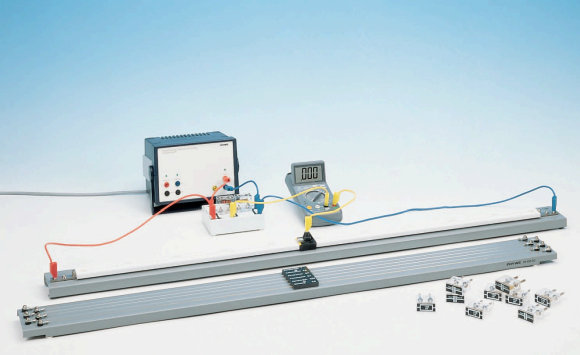
\includegraphics[width=0.45\textwidth]{IMAGES/wheatstone_bridge.png} % Replace with actual image path
    \caption{Wheatstone Bridge Experimental Setup \cite{lab_manual}.}
    \label{fig:setup}
\end{figure}

\section{Procedure}
To perform the experiment, the circuit was set up as shown in Figure~\ref{fig:setup}
, utilizing a Wheatstone Bridge configuration. 
Different known resistors \( R_2 \) were used, and the slider was adjusted 
along the resistance wire until the galvanometer indicated zero current
, signaling a balanced bridge. At this point, the corresponding lengths \( L_2 \) and \( L_3 \) were recorded. 
The unknown resistance \( R_1 \) was calculated using the equilibrium 
condition of the Wheatstone Bridge, as shown in Eq.~\ref{eq:wheatstone}. This procedure was initially performed for various resistors, and as an example, the resistivity was specifically calculated for a wire with a diameter of 0.5 mm, using its length and measured resistance. The calculation of resistivity was based on the relationship presented in Eq.~\ref{eq:resistivity}.

\section{Results and Data}

\subsection{Measured Values}
Table~\ref{tab:results} presents the recorded lengths and calculated 
resistances for various configurations for known ($R_1$, $R_4$) resistances. The calculations were performed using 
the formulas derived in the previous sections, as documented in the 
\texttt{Calculations.ipynb} notebook \cite{github}.

\begin{table}[H]
\centering
\begin{tabular}{cccccc}
\hline
$R_1$ (k$\Omega$) & $R_4$ (k$\Omega$) & $L_2$ (cm) & $L_3$ (cm) & $\frac{R_1}{R_2}$ & $\frac{L_2}{L_3}$\\
\hline
4.7 & 10 & 31.6 & 68.4 & 0.47 & 0.462 \\
0.330 & 0.150 & 68.6 & 31.4 & 2.2 & 2.185\\
\hline
\end{tabular}
\caption{Measured values of resistances and lengths.}
\label{tab:results}
\end{table}

\begin{figure}[H]
    \centering
    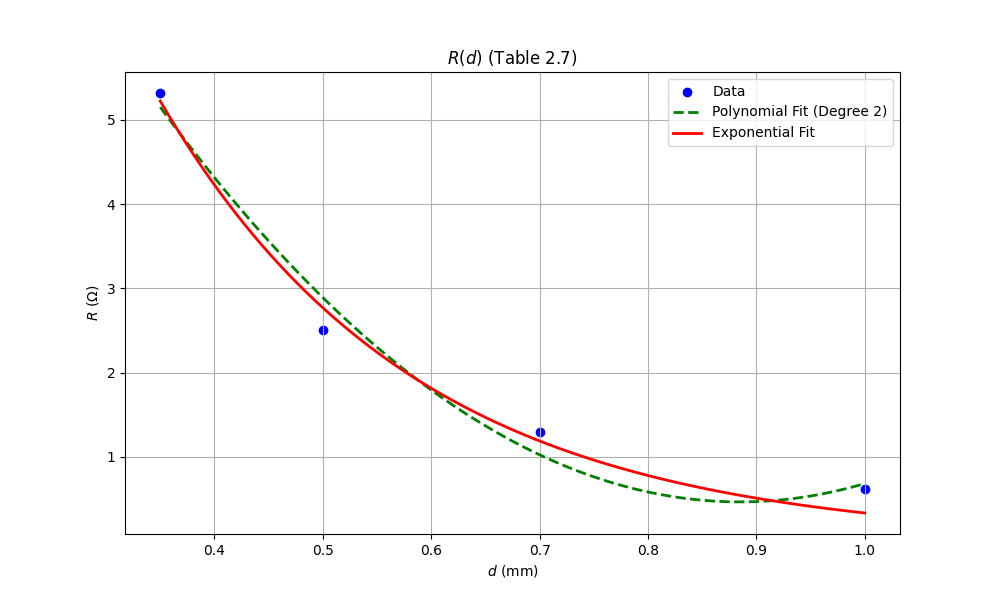
\includegraphics[width=0.45\textwidth]{output_plots/resistance_vs_diameter_table_2_7.png} % Replace with actual image path
    \caption{Plot of Resistance vs. Diameter based on experimental values \cite{lab_manual}. The graph is also hand-drawn on millimetric paper, available in the report appendix or repository \cite{graphonmillimetricpaper}.}
    \label{fig:resistance_vs_diameter}
\end{figure}

\subsection{Resistivity Calculation}
As an example, the resistivity (\(\rho\)) of a wire with a diameter of 0.5 mm was calculated using its measured resistance and length. The resistance for this wire was determined to be approximately \(2.770 \, \Omega\) for a length of \(100 \, \text{cm}\). The resistivity values for this wire, along with the calculations from the notebook, are summarized in Table~\ref{tab:resistivity}.

Using the resistivity formula, we find:
\[
\rho = \frac{R \cdot \pi \cdot \left(\frac{d}{2}\right)^2}{L}
\]
The calculated resistivity is approximately \(5.44 \times 10^{-5} \, \Omega \cdot \text{cm}\).

\begin{table}[H]
\centering
\begin{tabular}{ccc}
\hline
Diameter (mm) & Length (cm) & $\rho$ ($\Omega\cdot$cm)\\
\hline
0.5 & 100 & \(5.44 \times 10^{-5}\) \\ % Calculated resistivity value
\hline
\end{tabular}
\caption{Resistivity values for the wire with a diameter of 0.5 mm.}
\label{tab:resistivity}
\end{table}


\section{Discussion}
The Wheatstone Bridge provided accurate results, with experimental data closely aligning with theoretical values. Minor deviations may be due to measurement inaccuracies or contact resistance. The resistivity results match standard values, confirming the reliability of the Wheatstone Bridge for resistivity measurements.

\section{Conclusion}
This experiment successfully applied the Wheatstone Bridge method to determine unknown resistance and measure resistivity. Results support the theory, showcasing the Wheatstone Bridge's precision for such measurements.


\section{Additional Resources}
For detailed information, including the Lab Manual, source code, and related experiments, visit the GitHub repository provided below or scan the QR code in Fig.~\ref{fig:qr}.

\begin{thebibliography}{9}
\bibitem{lab_manual}
    ISTANBUL UNIVERSITY, 
    \textit{Physics Laboratory II Experiment Book: Electricity and Magnetism}, 
    Department of Physics, 2024.

\bibitem{github}
    \textit{Source code and additional experiments are available in the GitHub repository.} \\ 
    Access it at: \url{https://github.com/ibeuler/LAB-Reports}

\end{thebibliography}

\begin{figure}[H]
    
    \centering
    \begin{minipage}{0.15\textwidth}
        \centering
        \qrcode[height=2cm]{https://github.com/ibeuler/LAB-Reports}
    \end{minipage}%
    \begin{minipage}{0.2\textwidth}
        \raggedright
        \caption{Access the GitHub repository for the lab manual, source code, and related experiments: \href{https://github.com/ibeuler/LAB-Reports}{\url{https://github.com/ibeuler/LAB-Reports}}.}
    \end{minipage}
    \label{fig:qr}
\end{figure}
\end{document}
